
\chapter{成果与对比}

\section{成果展示}

本文着重对系统的架构进行了介绍,同时也实现了一个功能完整,包含全部文章中所提到技术和功能点,以及符合文中陈述的开发框架的清华大学工会管理系统,以此来证明文中所述的系统架构能够投入到实际运用,是行之有效的工程系统框架。

\subsection{B/S浏览器端}

接下来将通过一系列的图片和描述来模拟开展一个公会活动的过程。

首先,总工会主席需要通过上传一份公会人员名单来创建一个群组。图\ref{fig:postTarget}展示了工会主席创建工会人员群组的过程。

\begin{figure}[H]
  \centering
  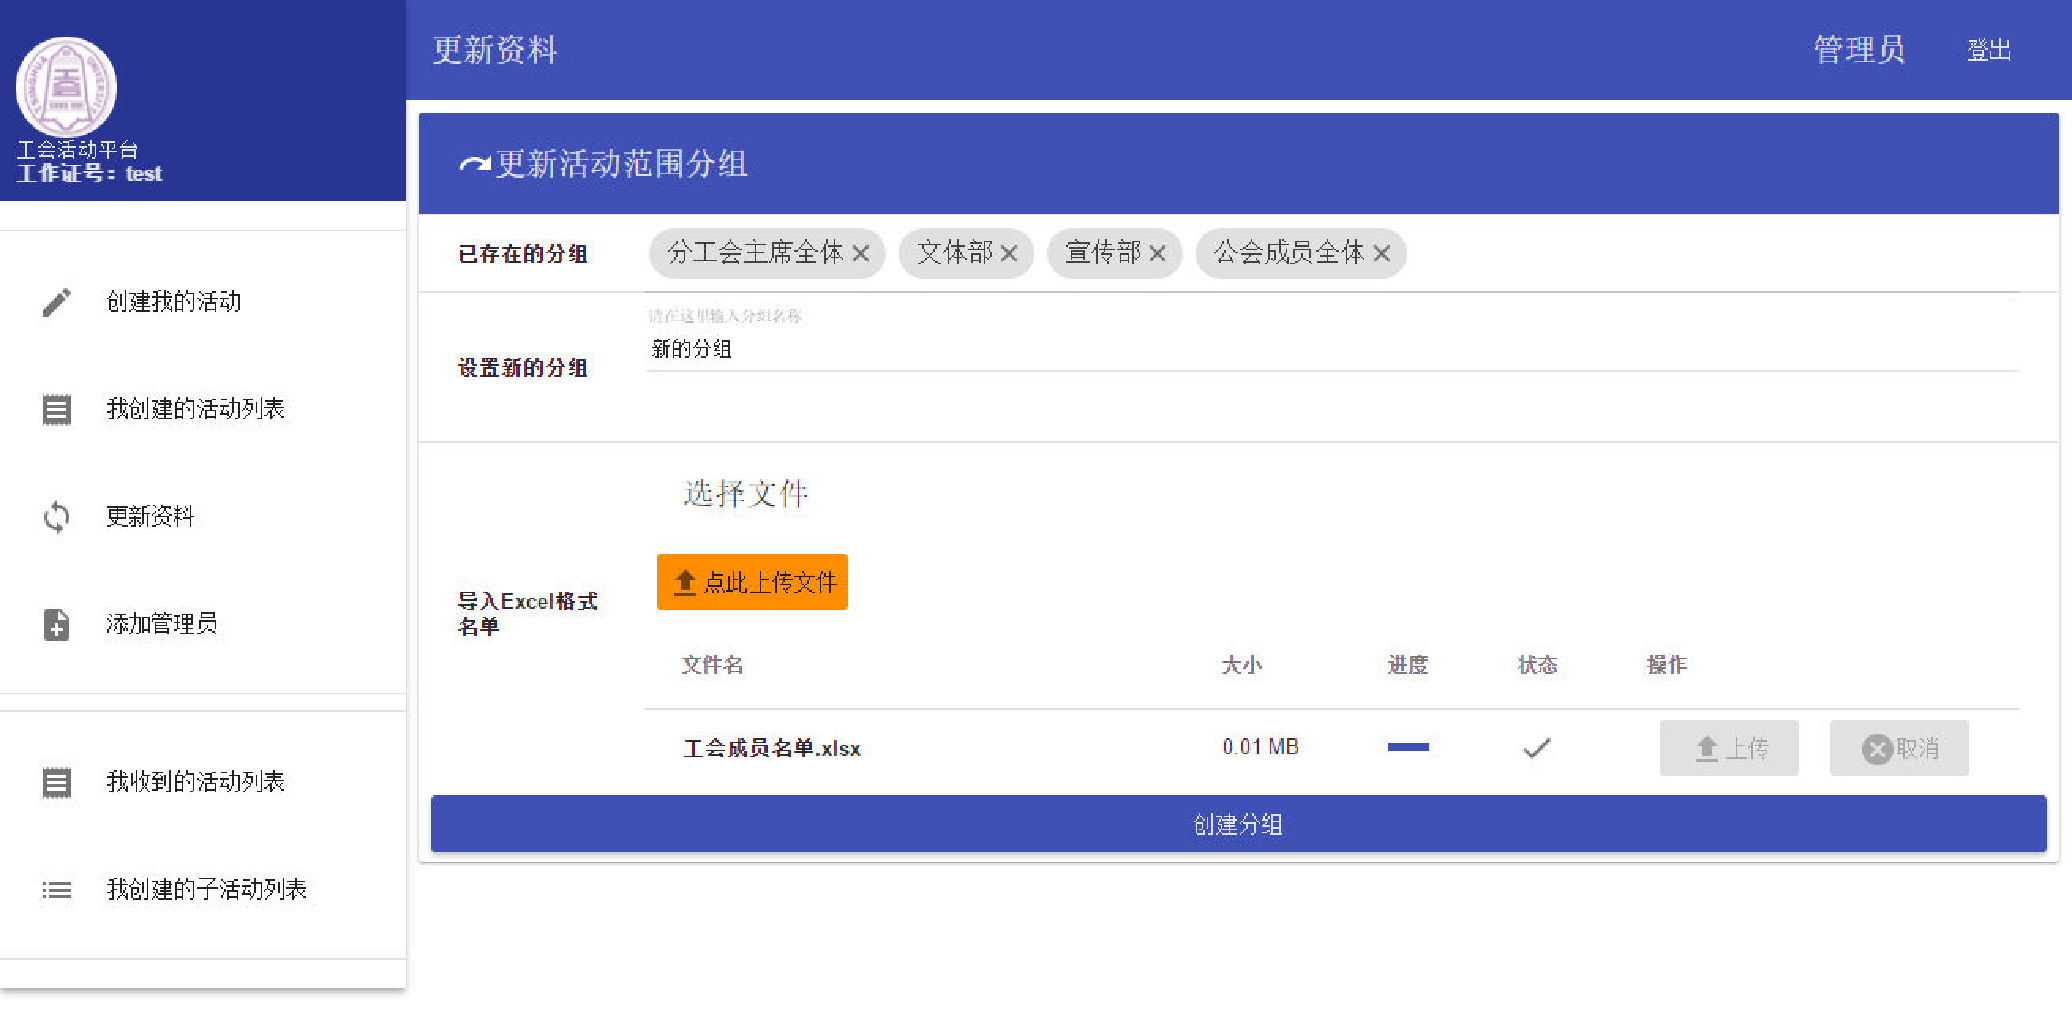
\includegraphics[width=0.8\textwidth]{postTarget.pdf}
  \caption{总工会主席创建群组}
  \label{fig:postTarget}
\end{figure}

在完成了群组创建过程之后,工会主席就可以创建一个新的活动并且指定刚刚创建的群组作为活动通知下达的对象进行发送。图\ref{fig:createEvent}展示了工会主席创建活动时的界面。

\begin{figure}[H]
  \centering
  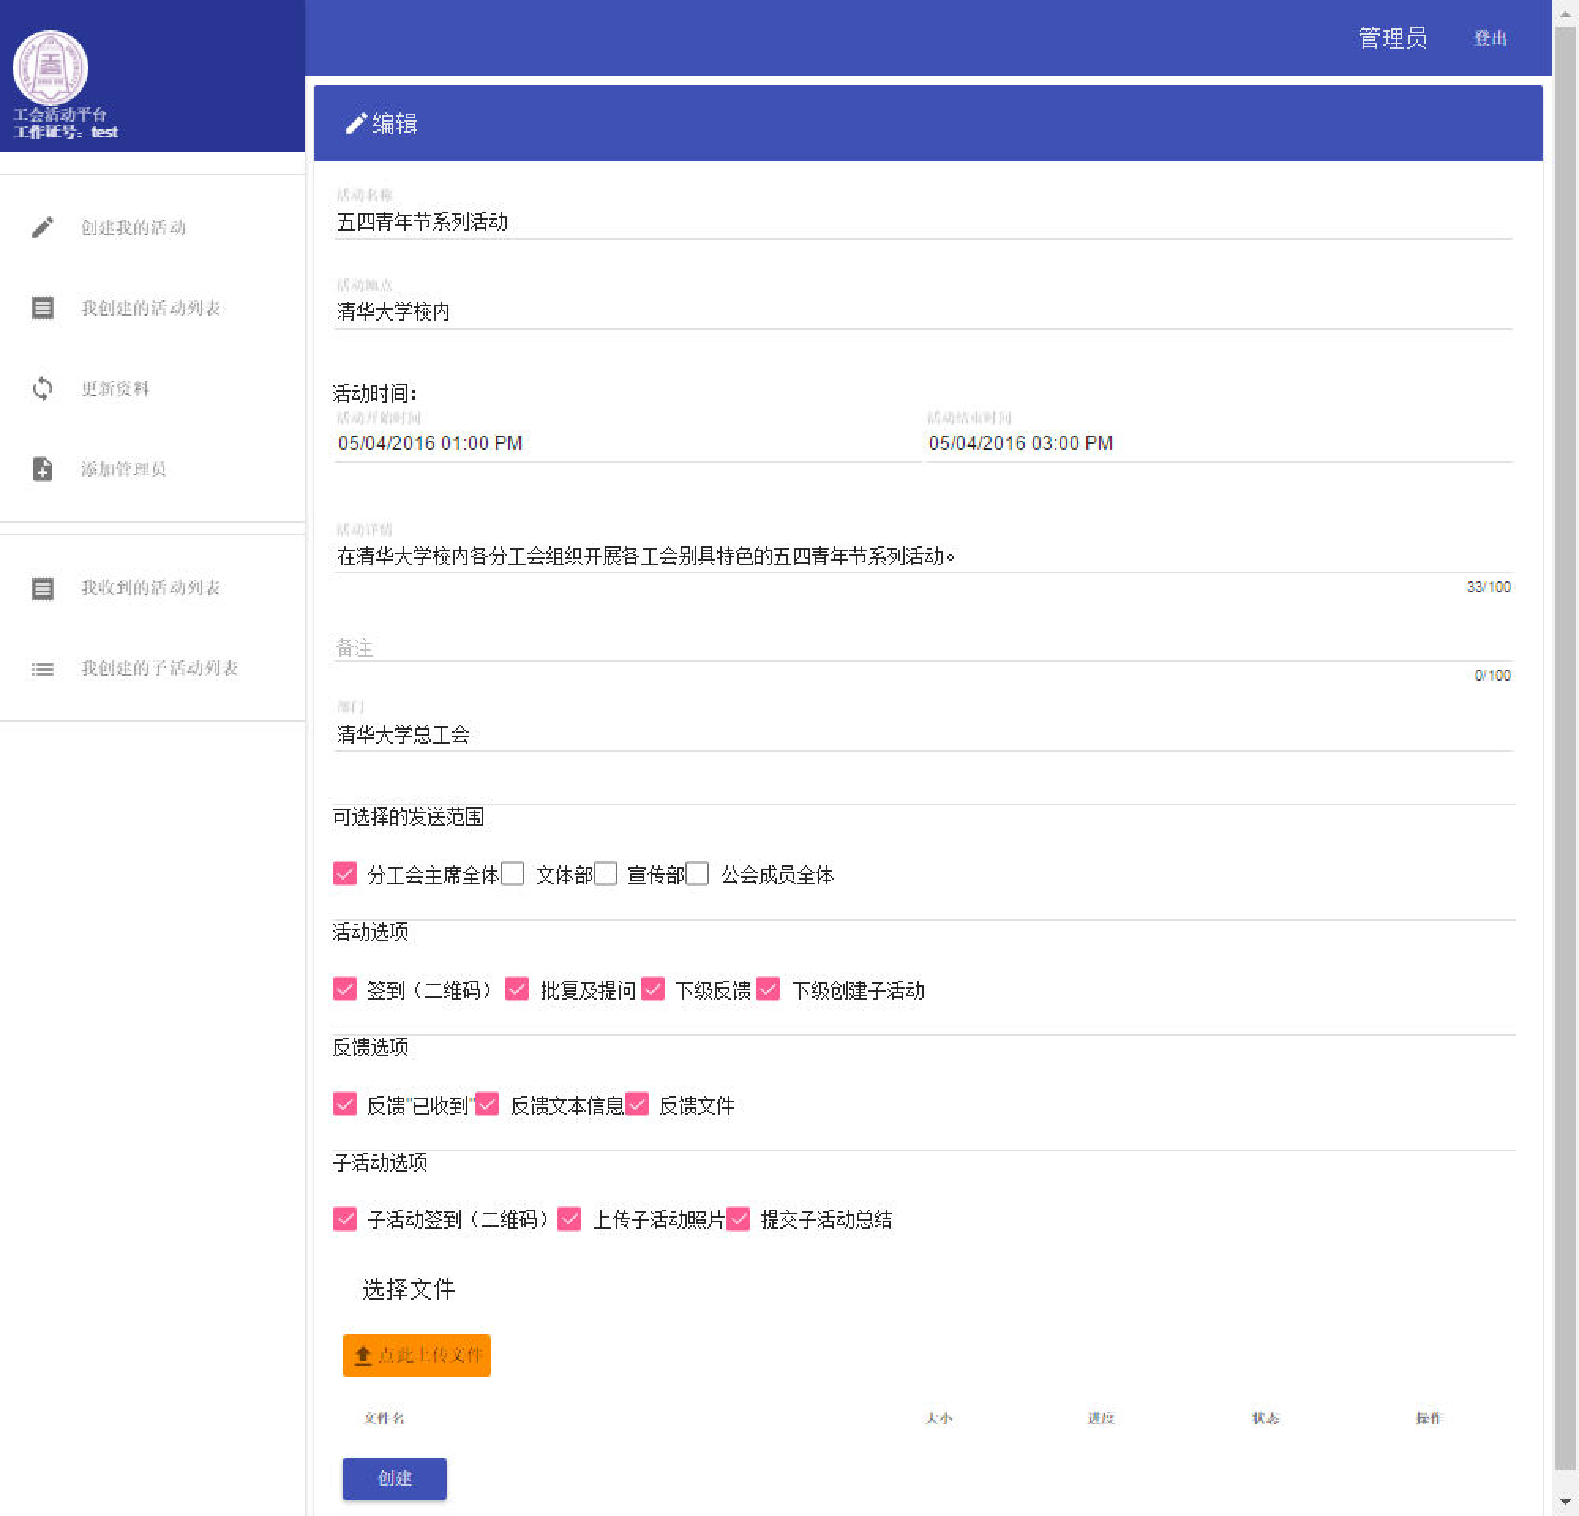
\includegraphics[width=0.8\textwidth]{createEvent.pdf}
  \caption{总工会主席创建一个新的活动}
  \label{fig:createEvent}
\end{figure}

完成活动创建之后,工会主席就能够在图\ref{fig:eventList}中查看到自己创建的活动列表了。

\begin{figure}[H]
  \centering
  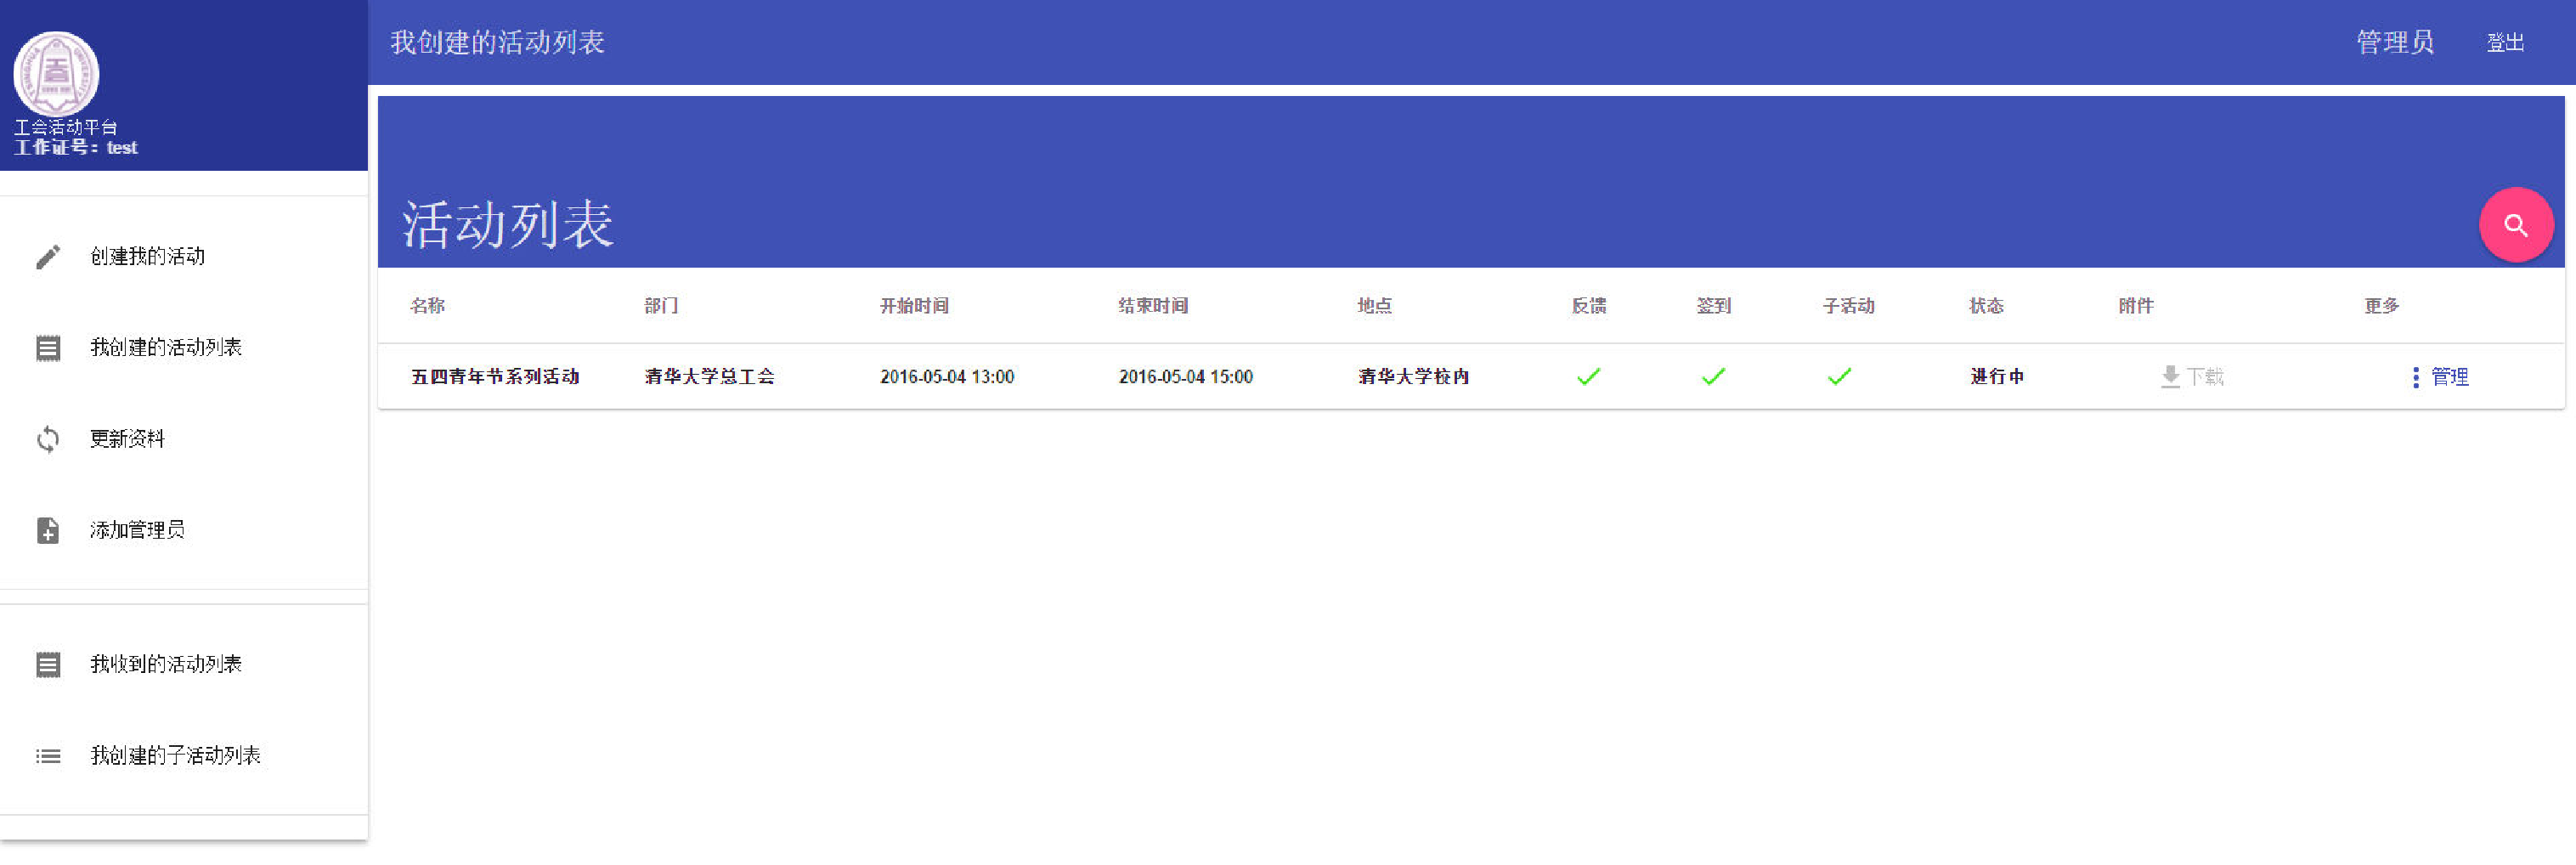
\includegraphics[width=0.8\textwidth]{eventList.pdf}
  \caption{总工会主席创建的活动列表}
  \label{fig:eventList}
\end{figure}

此时收到这个活动的分工会主席就可以登录到系统中并查看到自己已经收到了这个活动的通知(图\ref{fig:activityList})。在图\ref{fig:activityDetail}所示收到的活动详情页中,分工会主席可以针对活动的需求来完成相应的工作。

\begin{figure}[H]
  \centering
  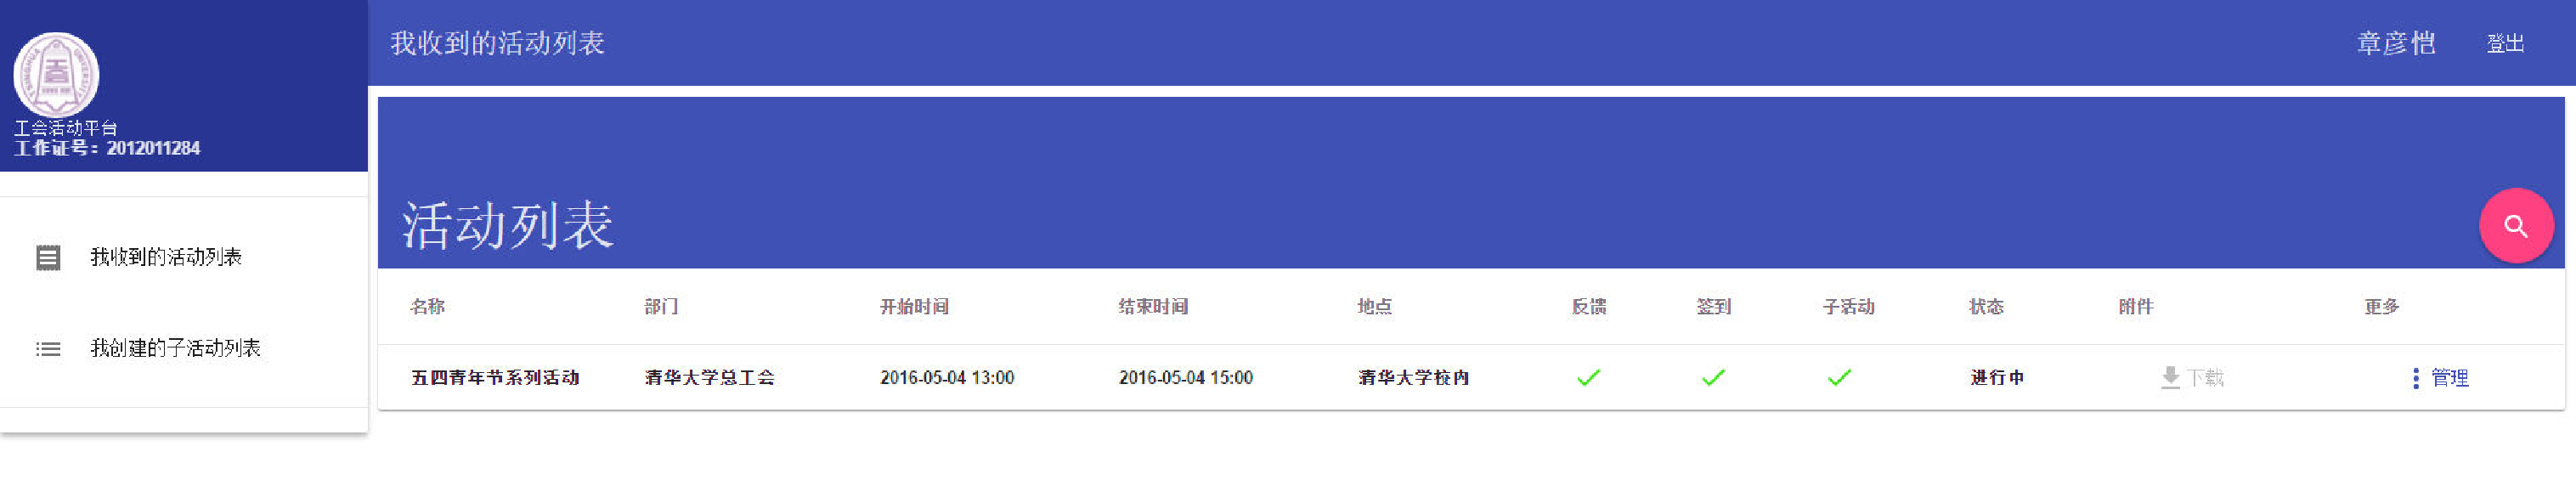
\includegraphics[width=0.8\textwidth]{activityList.pdf}
  \caption{分工会主席收到的活动列表显示}
  \label{fig:activityList}
\end{figure}

\begin{figure}[H]
  \centering
  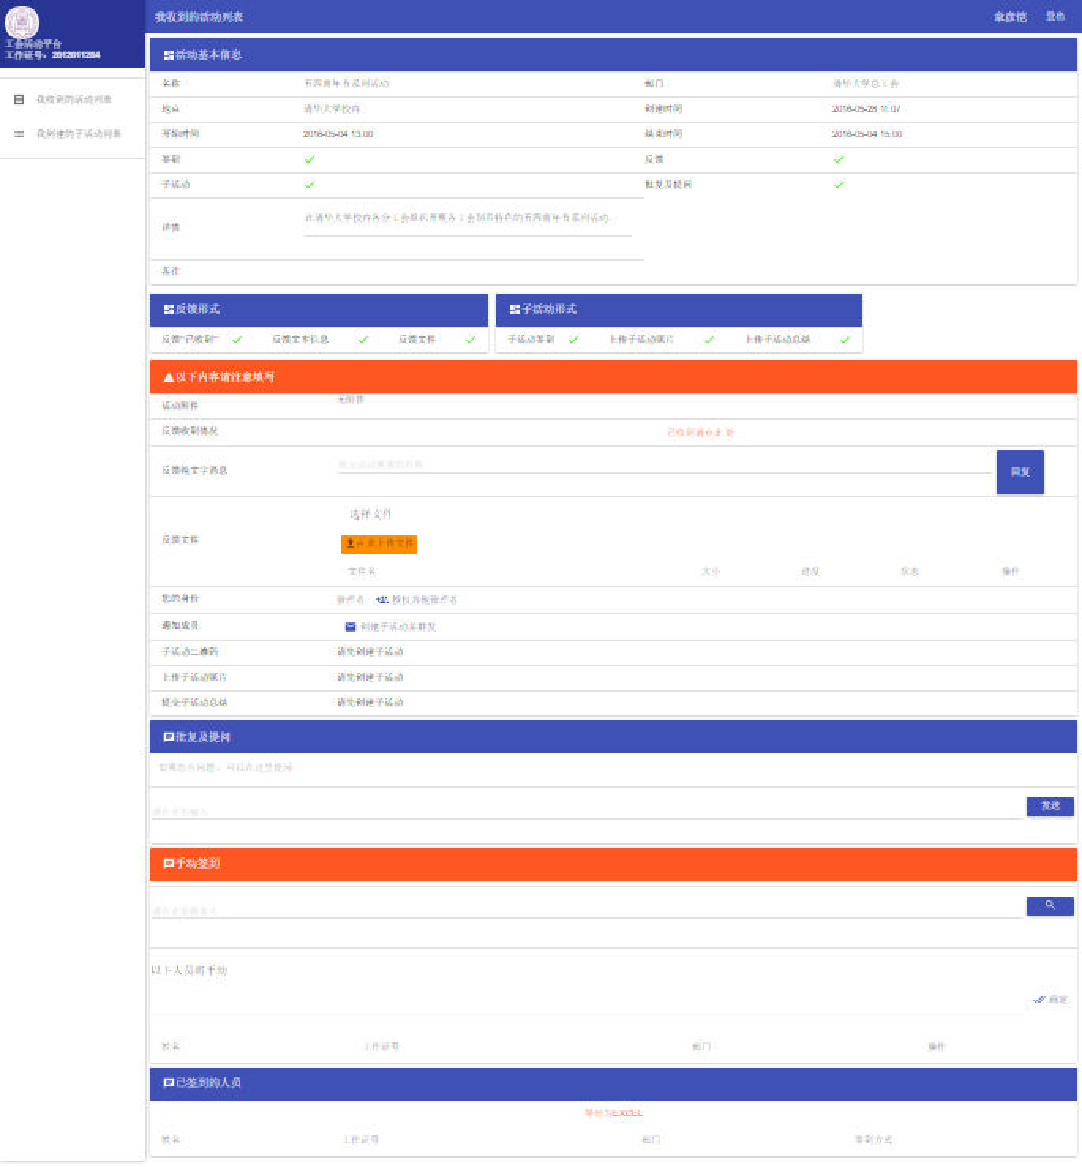
\includegraphics[width=0.8\textwidth]{activityDetail.pdf}
  \caption{分工会主席收到的活动详情页面}
  \label{fig:activityDetail}
\end{figure}

由于创建的活动需要分工会主席开展子活动,因此分工会主席需要点击“开展子活动”按钮,并填写子活动的详细信息(图\ref{fig:shotActivity})。

\begin{figure}[H]
  \centering
  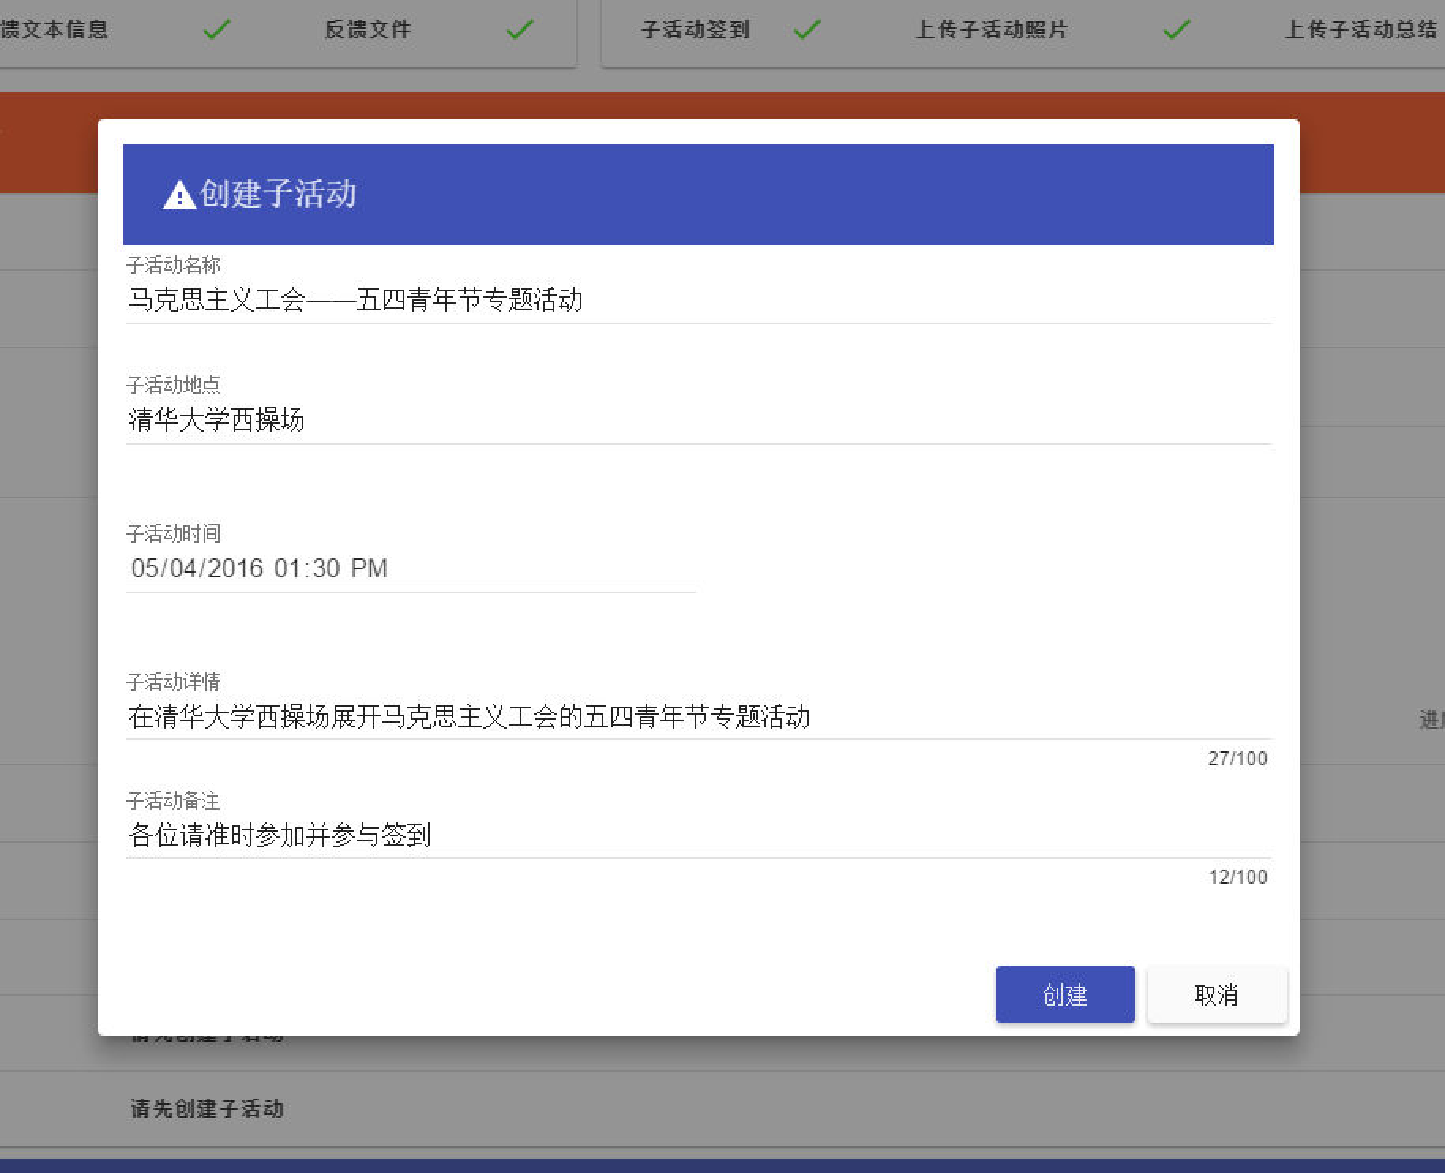
\includegraphics[width=0.8\textwidth]{shotActivity.pdf}
  \caption{分工会主席填写子活动详细信息并创建子活动}
  \label{fig:shotActivity}
\end{figure}

在完成子活动创建之后,工会成员就会收到新的可以参加的活动通知了,如图\ref{fig:shotPost}。

同时,分工会主席在详情页中可以就活动的需求向工会主席提出问题,工会主席可以对这些问题进行回答,如图\ref{fig:message}所示。

\begin{figure}[H]
  \centering
  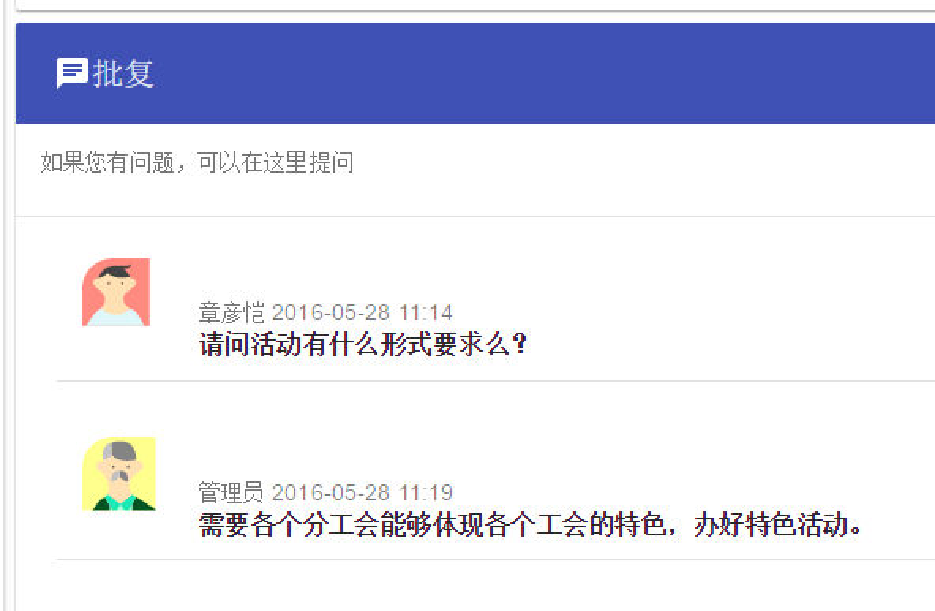
\includegraphics[width=0.8\textwidth]{message.pdf}
  \caption{分工会主席与工会主席通过系统进行提问和回答}
  \label{fig:message}
\end{figure}

当子活动的状态发生变化的时候,总工会主席可以在活动的详情页中看到该活动所有下属子活动以及活动本身的统计信息记录。图\ref{fig:eventDetail}即为“五四青年节系列活动”的详情页展示。

\begin{figure}[H]
  \centering
  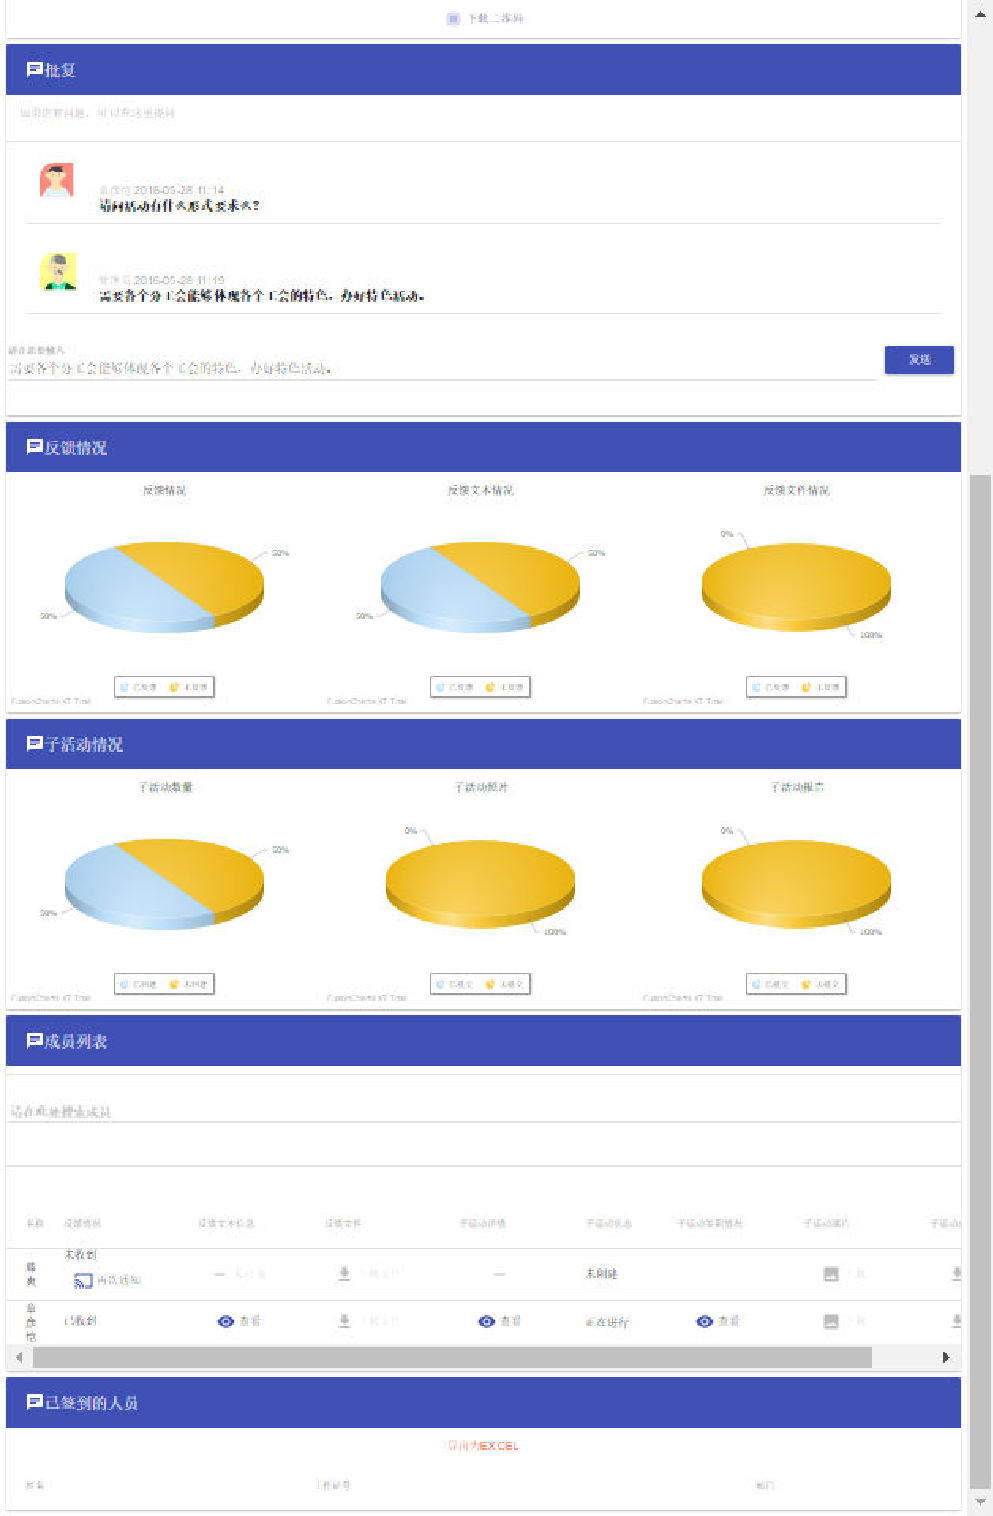
\includegraphics[width=0.8\textwidth]{eventDetail.pdf}
  \caption{工会主席在活动的详情页中看到的活动开展情况统计}
  \label{fig:eventDetail}
\end{figure}

在网页客户端中可以对一个活动进行手动签到。由于手动签到的效果和使用二维码进行签到的效果相似,因此将在\ref{section:wechat}中进行展示。

\subsection{C/S微信微平台}

\label{section:wechat}

图\ref{fig:shotPost}展示了清华大学工会微信微平台的界面。图\ref{fig:shotPost}是在微信的桌面客户端的界面截图。

\begin{figure}[H]
  \centering
  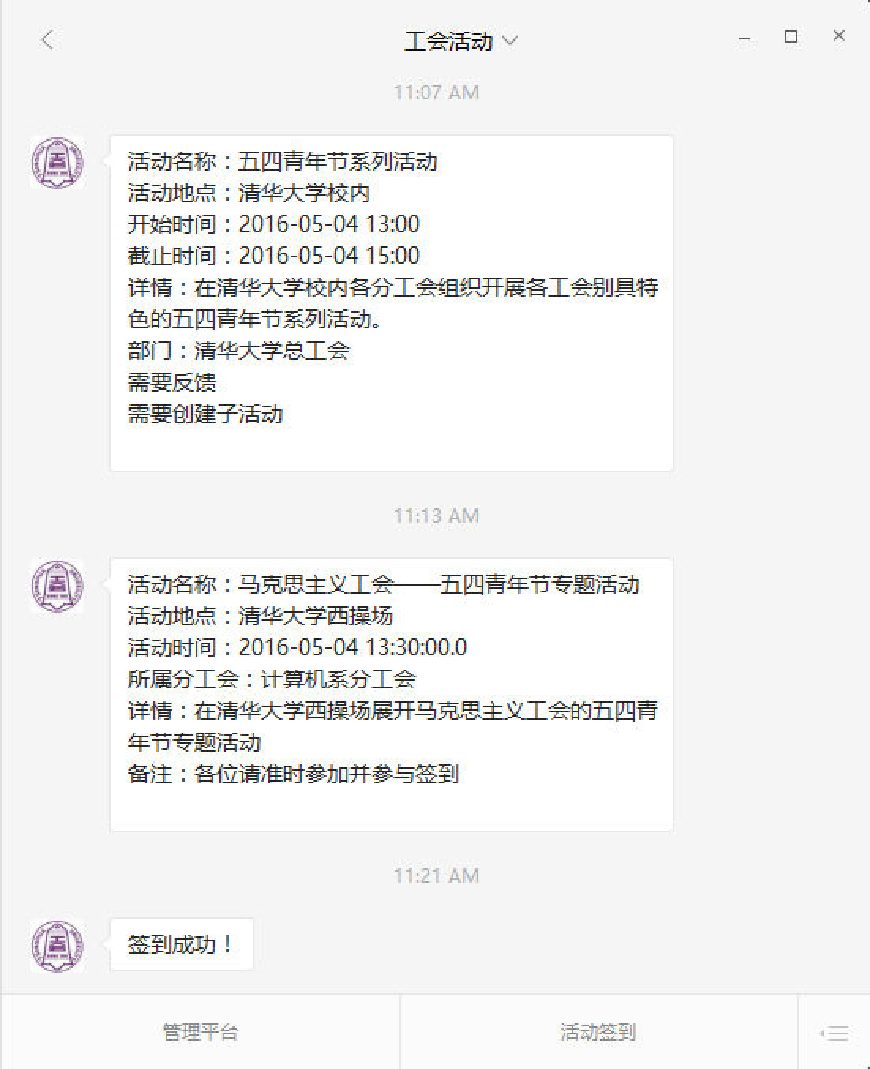
\includegraphics[width=0.8\textwidth]{shotPost.pdf}
  \caption{清华大学工会微信微平台界面}
  \label{fig:shotPost}
\end{figure}

当用户单击管理平台按钮之后,会进入到管理平台界面。通过管理平台,用户可以通过简单的操作对活动和子活动进行查看和管理,如图\ref{fig:shotWechatMenu}所示。

\begin{figure}[H]
  \centering
  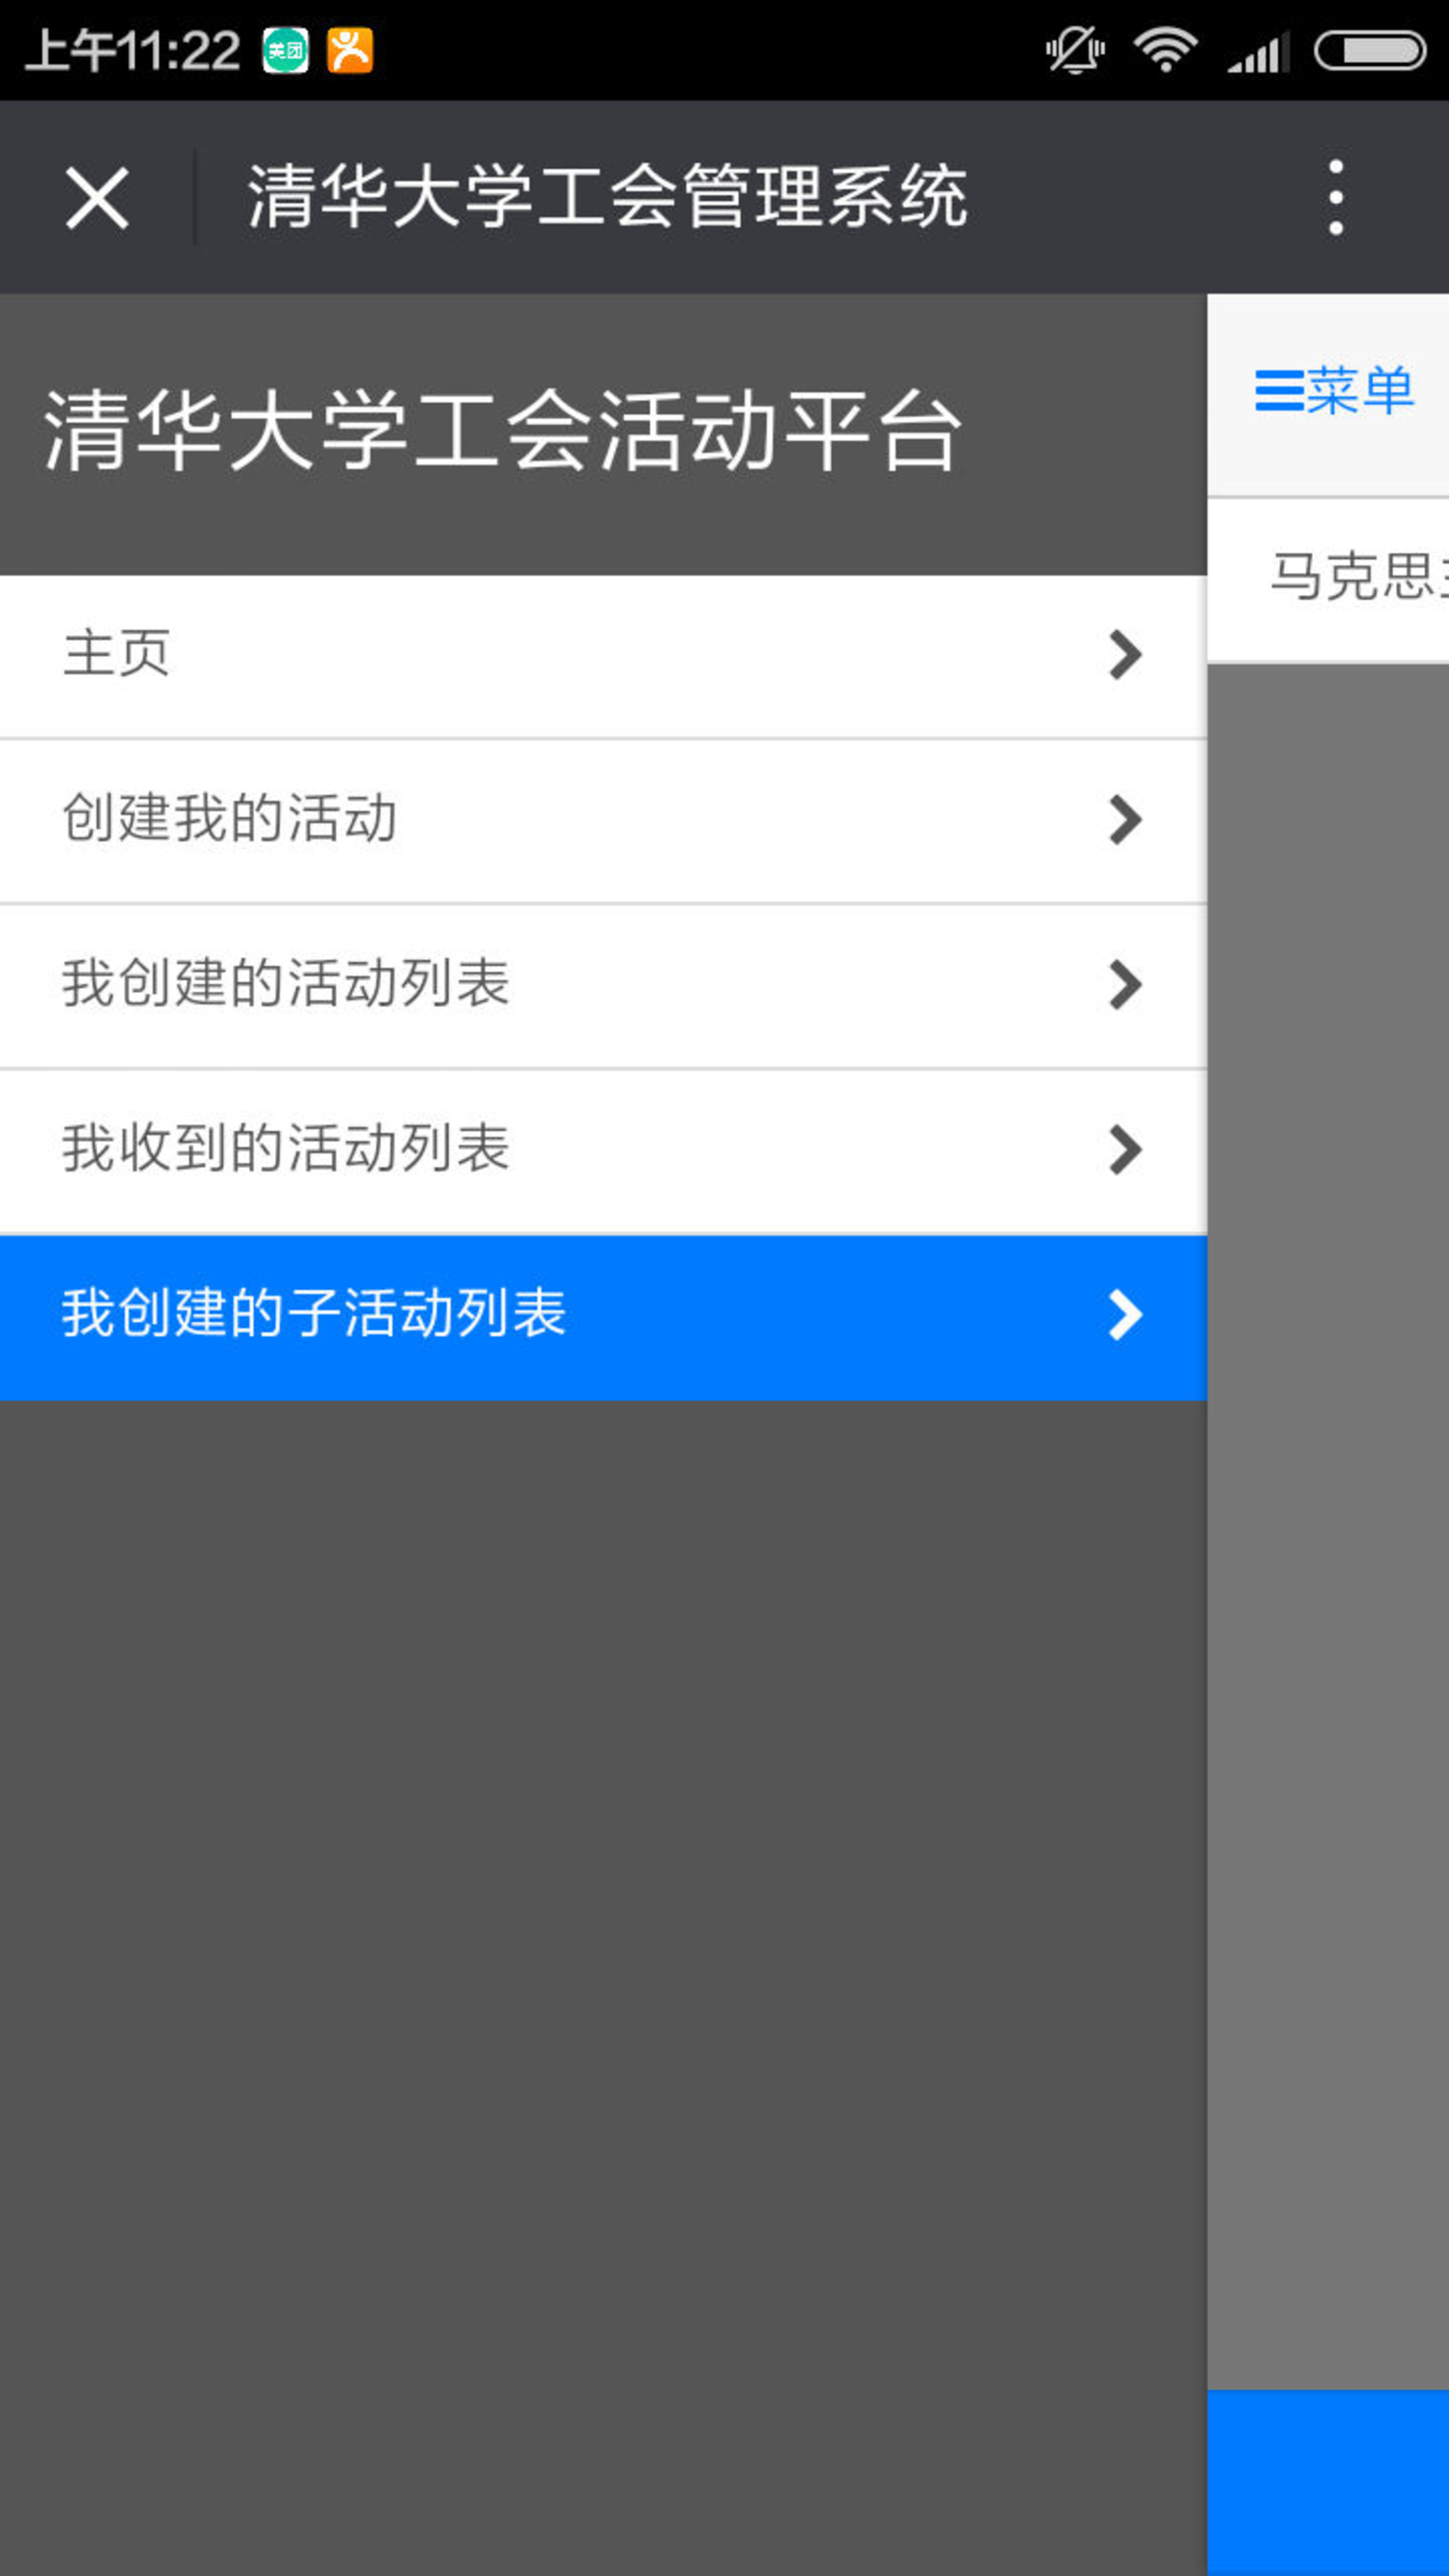
\includegraphics[width=0.5\textwidth]{shotWechatMenu.pdf}
  \caption{清华大学工会微信微平台管理平台界面}
  \label{fig:shotWechatMenu}
\end{figure}

进入收到的子活动,并选择相应的子活动栏目,就可以看到子活动的详细信息了(图\ref{fig:shotWechatDetail})。

\begin{figure}[H]
  \centering
  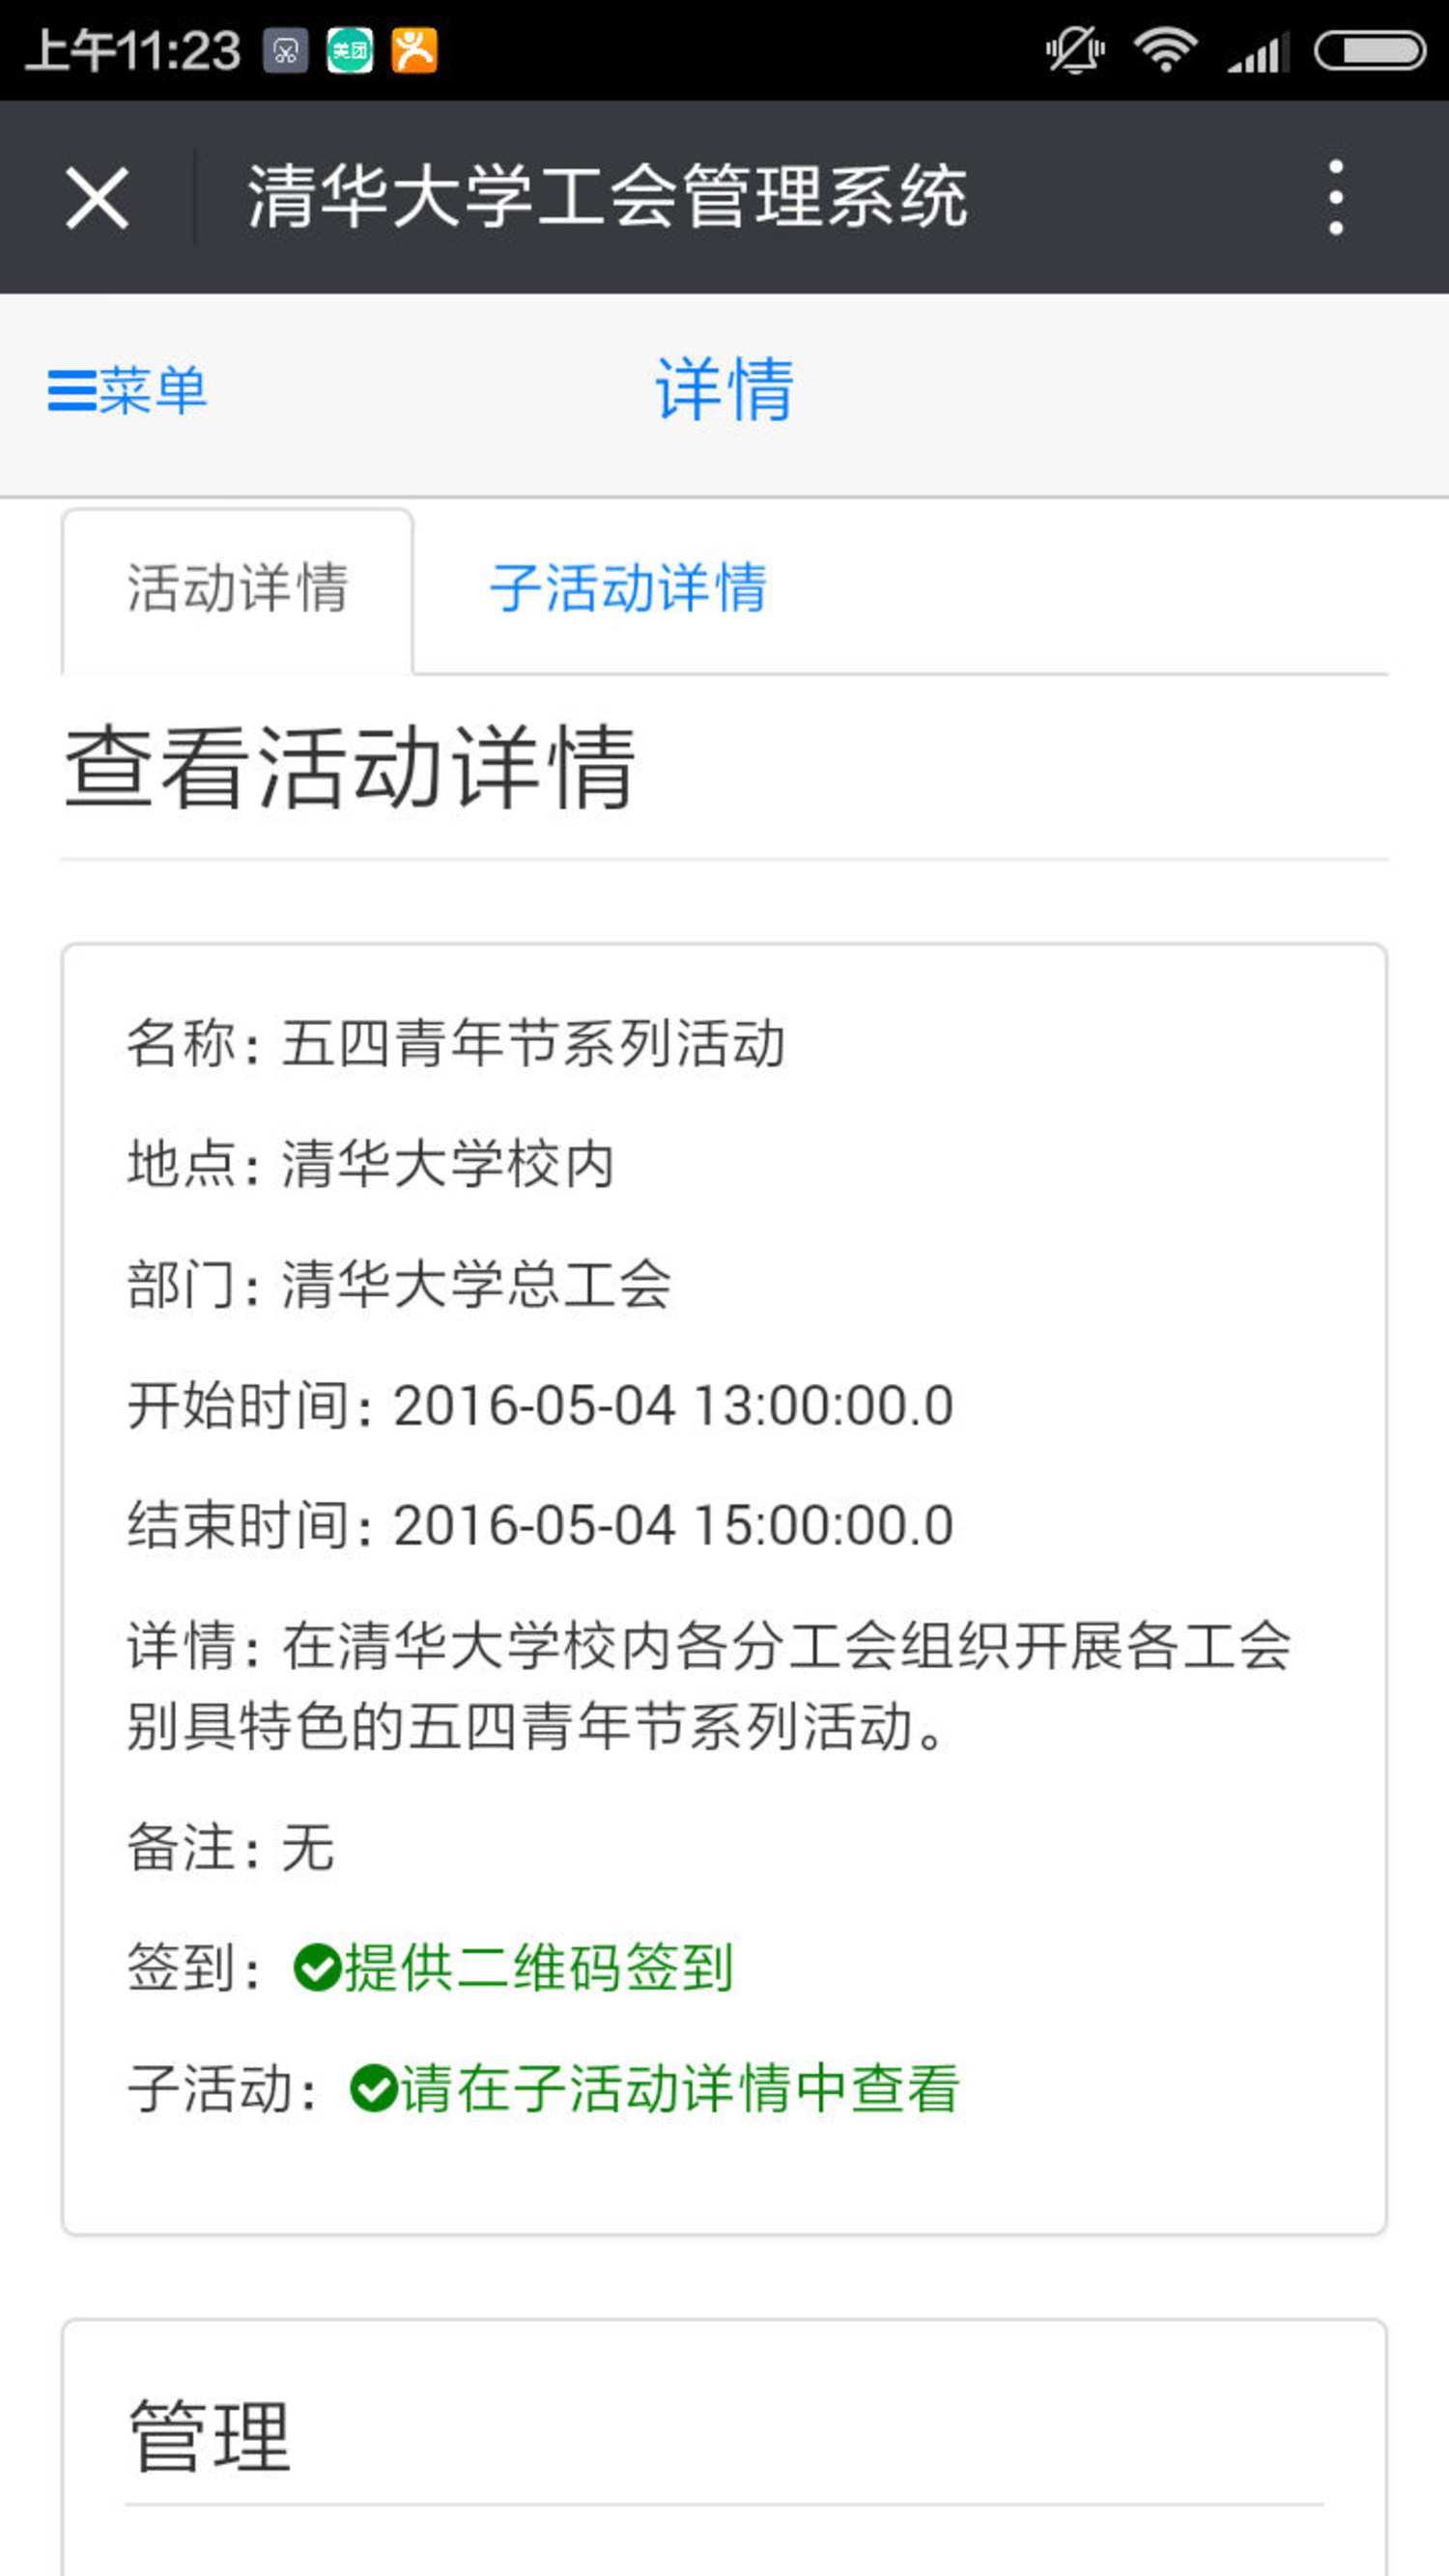
\includegraphics[width=0.5\textwidth]{shotWechatDetail.pdf}
  \caption{在工会微信管理平台查看子活动的详情}
  \label{fig:shotWechatDetail}
\end{figure}

除了能够查看子活动的详情以外,还能够在管理平台中对子活动进行方便的一键操作管理(图\ref{fig:shotWechatManage})。

\begin{figure}[H]
  \centering
  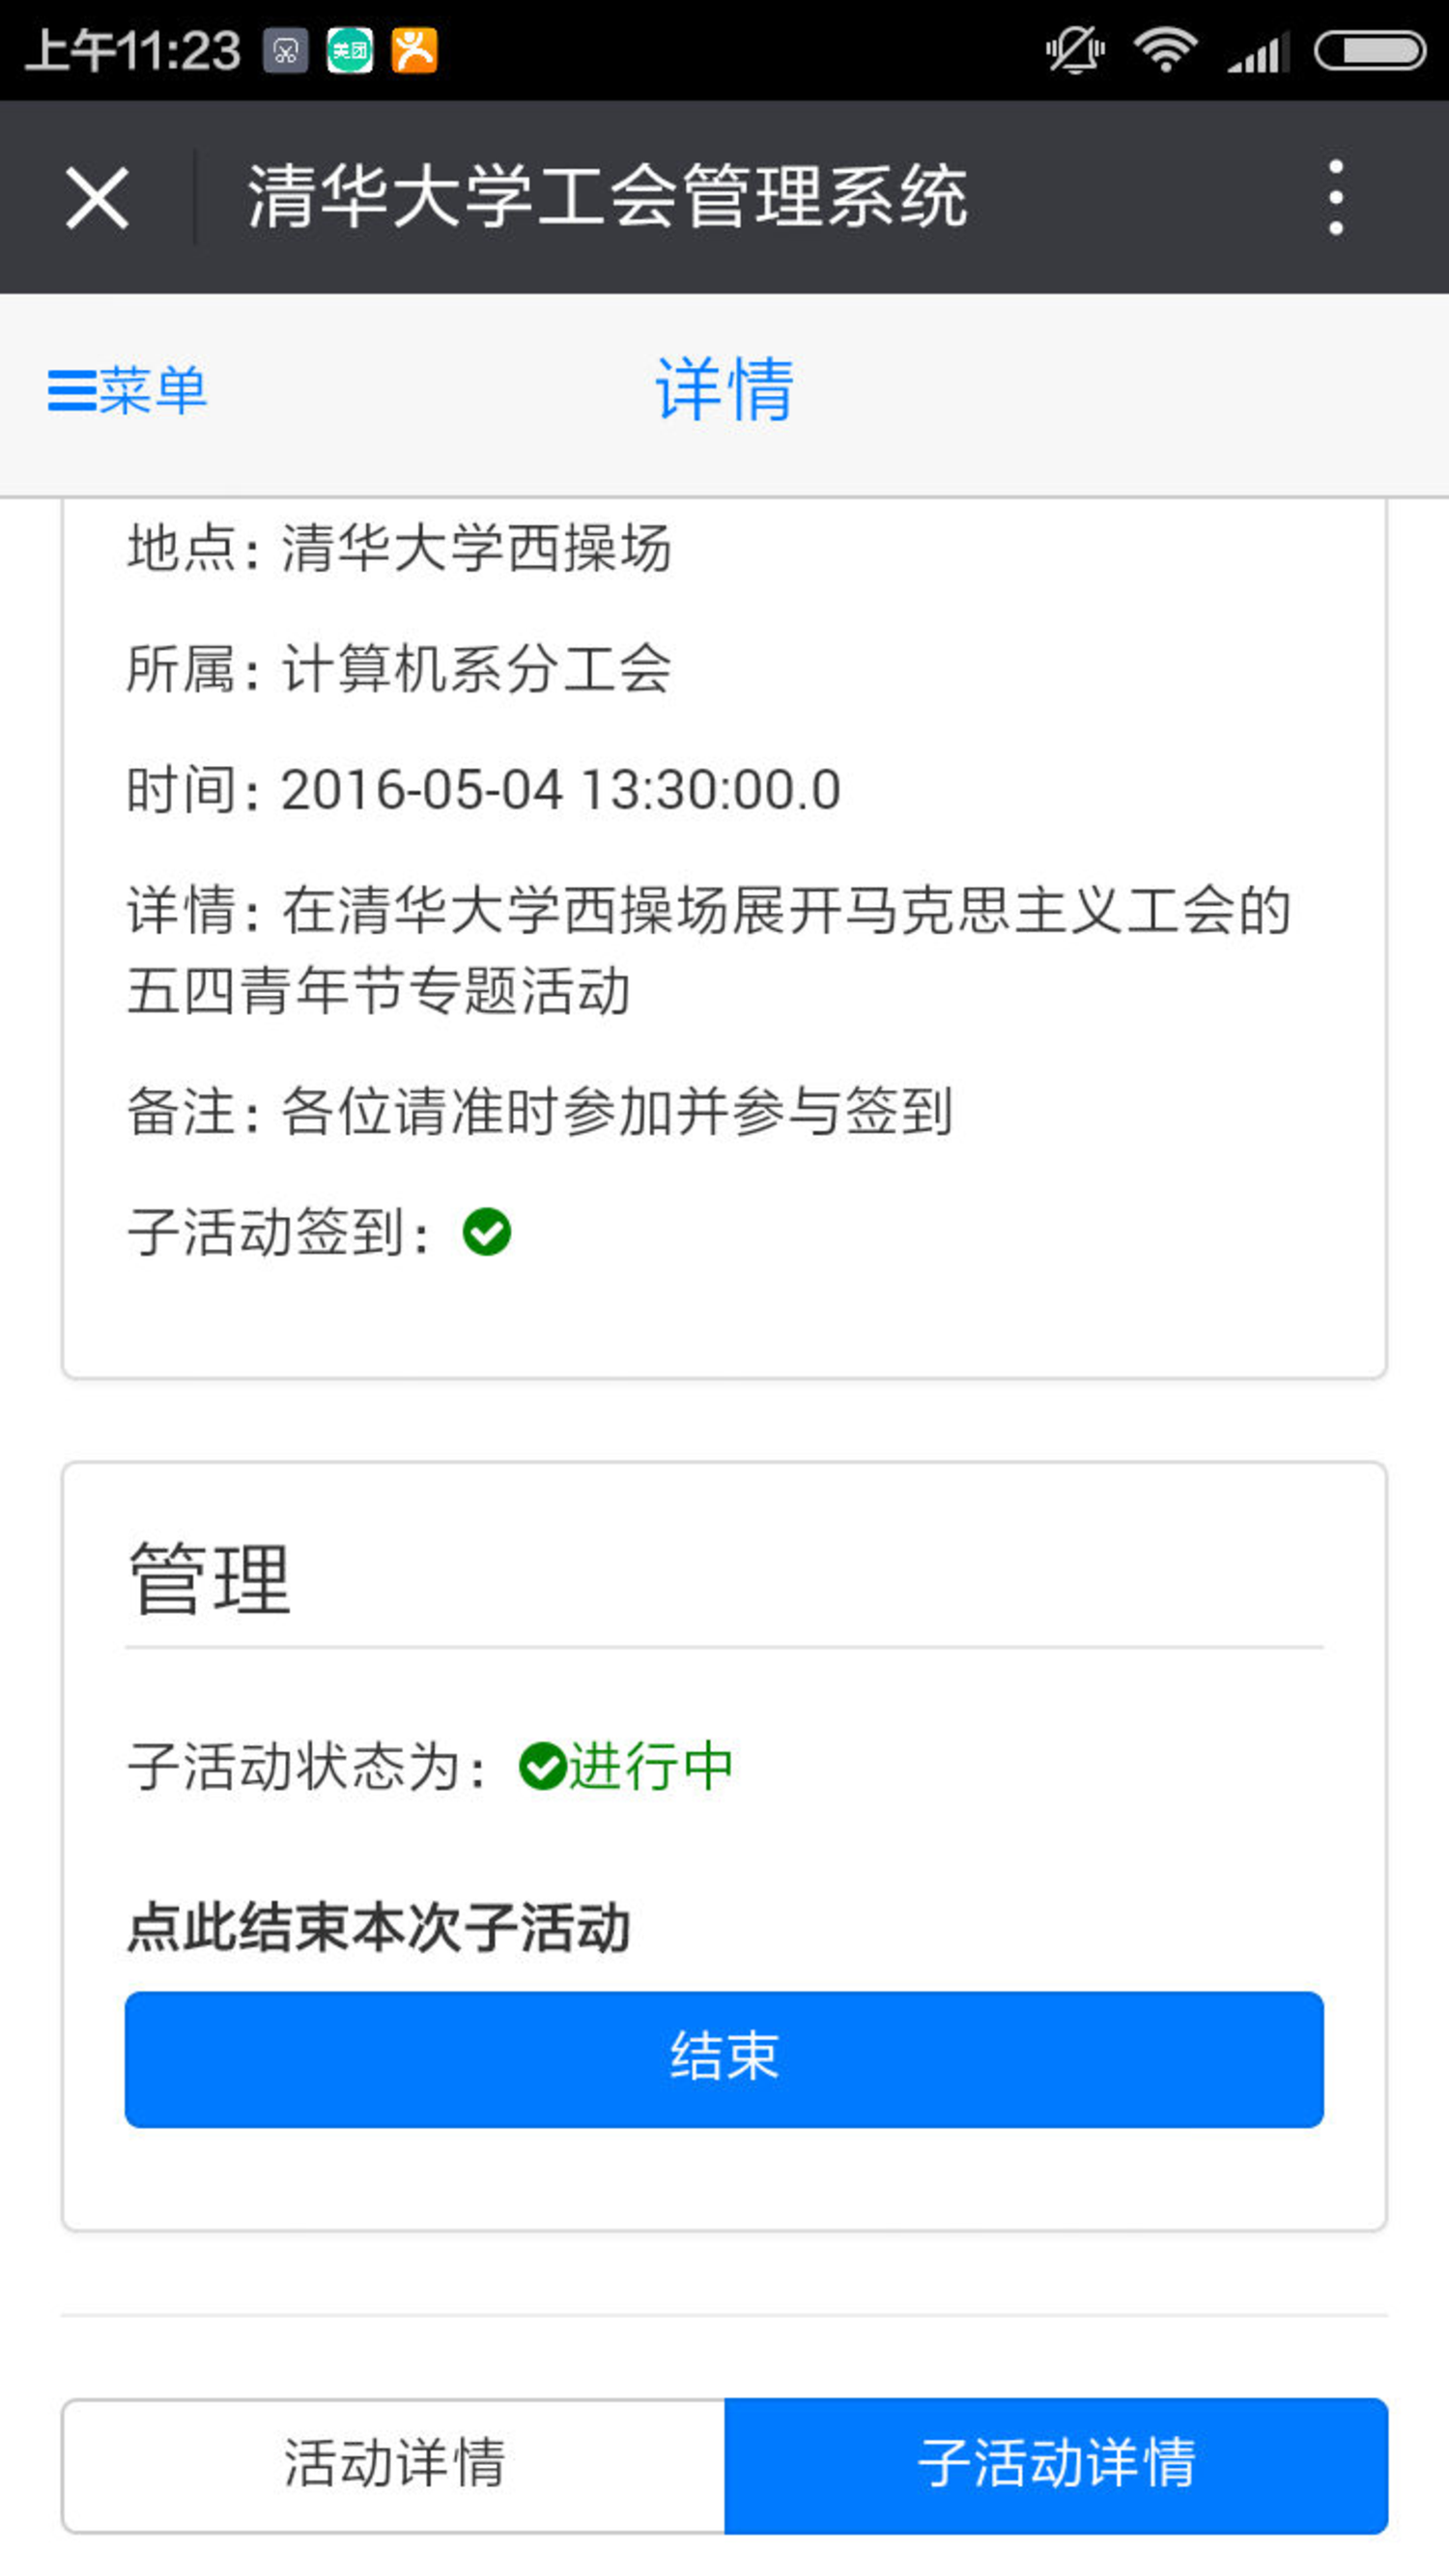
\includegraphics[width=0.5\textwidth]{shotWechatManage.pdf}
  \caption{在工会微信管理平台对子活动进行管理}
  \label{fig:shotWechatManage}
\end{figure}

\section{对比和评价}

在这一节中,我们将分别对清华大学工会管理系统的功能和性能进行定性和定量的评价。

\subsection{功能评价}

我们将清华大学工会管理系统与传统C/S行政系统、单纯B/S行政系统、基于HTTPS协议的B/S系统、基于微信公众号的C/S系统和基于移动应用的行政系统进行功能点对比。对比的功能点有:跨平台性,便携性,数据安全性,可用于行政系统目的,以及消息推送。评价结果见表\ref{table:compare}。


\begin{table}
  \centering
  \caption{不同平台系统的对比评价}
  \label{table:compare}
    \begin{tabular}{lccccc}
      \toprule
      系统 & 跨平台性 & 便携性能 & 数据安全 & 行政目的 & 消息推送 \\
      \midrule % $\surd$
      清华大学工会管理系统 		&$\surd$ &$\surd$ &$\surd$ &$\surd$ &$\surd$ \\
      传统C/S行政系统 			& & & &$\surd$ & \\
      单纯B/S行政系统 			&$\surd$ & & &$\surd$ & \\
      基于HTTPS协议的B/S系统 	&$\surd$ & &$\surd$ &$\surd$ & \\
      基于微信公众号的C/S系统 	&$\surd$ &$\surd$ & & &$\surd$ \\
      基于移动应用的行政系统 	& &$\surd$ & ? & $\surd$ & $\surd$\\
      \bottomrule
    \end{tabular}
\end{table}

从表\ref{table:compare}中可以看到,传统的C/S行政系统除了可以用于行政目的以外,已经无法跟上时代对行政系统的要求。在当今的多平台环境下,它已经逐渐被人们所淘汰。而单纯的B/S行政系统没有利用最近移动设备的发展给用户带来的便利,对于清华大学工会活动管理系统来说,无法进行及时的消息推送,同时数据的安全性也存在问题。虽然数据的安全问题可以通过使用HTTPS协议来保证,然而其缺乏移动设备上的支持和推送功能仍然使得它的应用范围受限。而基于微信公共号的新型C/S系统虽然可以充分利用到移动设备的便携性质,但是用于行政目的需要输入信息的时候,移动设备还是会不可避免地受到输入方式的限制,而且对文件的操作和处理存在很大的困难。对于微信公众号来说,信息的呈现形式也会受到很大的局限,只能借助微信平台的有限呈现模式来呈现信息。因此用单一的微信公众号作为行政系统的主体是不合适的。而基于移动应用的行政系统首先会要求用户安装相应的移动应用,并且移动应用不可避免地会遇到和微信公众号相同的问题。虽然移动应用可以通过对数据加密来满足数据的安全性,但是其存在的局限性仍然限制了它作为行政系统主体的能力。

可以看到,结合了B/S和C/S的优点,再加上对微信移动平台的充分运用,使得文中的清华大学工会管理系统不仅可以借助移动设备推送的能力满足工会活动通知的及时性,同时利用网页浏览器客户端使得信息的控制和管理更加高效灵活。

\subsection{性能评价}

通过对清华大学工会管理系统进行压力测试可以很好地描述出一个系统的性能。压力测试的后端运行环境如表\ref{table:hardware}所示。

\begin{table}
  \centering
  \caption{压力测试后端运行环境表}
  \label{table:hardware}
    \begin{tabular}{ll}
      \toprule
      项目 & 参数 \\
      \midrule % $\surd$
      计算机型号 & Lenovo Y510p \\
      CPU & Intel(R) Core i7-4700MQ @ 2.40 GHz \\
      硬盘 & SAMSUNG Spinpoint M8 ST1000LM024 @ 5400 RPM \\
      物理内存 & 8.00 GB \\
      操作系统 & Windows 10 Enterprise 64-bit \\
      Tomcat版本 & Apache Tomcat 7.0.55 \\
      MySQL版本 & mysql Ver 14.14 Distrib 5.6.20\\
      JAVA版本 & Java(TM) SE Runtime Environment (build 1.8.0\_73-b02)\\
      \bottomrule
    \end{tabular}
\end{table}


压力测试的内容是模拟不同数量的用户同时对系统进行1000次操作。测试的第一部分是将两个查询操作打包组成一组操作,并重复1000次,以此来测试平台在数据不进行修改的情况下的抗压能力。测试的第二部分是将一次插入操作和一次查询操作打包组成一组操作,并重复一千次,以此来考察当平台中的数据数量不断增大的时候,平台应对大量并发的操作时的相应时间。图\ref{fig:pressure}展示了压力测试的结果。

\begin{figure}[H]
  \centering
  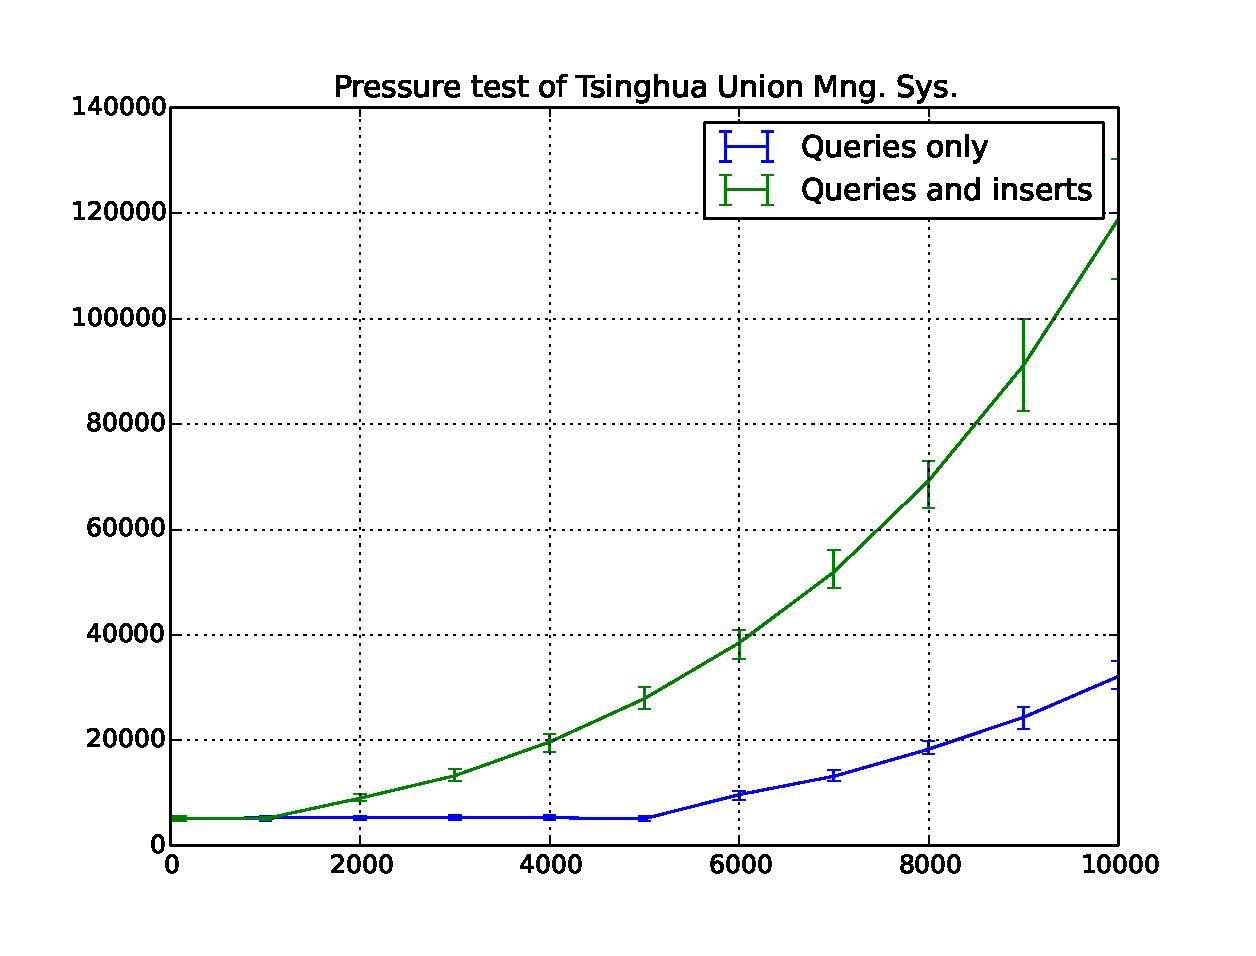
\includegraphics[width=0.8\textwidth]{pressureTest}
  \caption{压力测试结果图}
  \label{fig:pressure}
\end{figure}

图\ref{fig:pressure}中,横坐标为用户的数量,纵坐标为服务器的平均响应时间(单位:微秒)。从图中可以看到,在用户数量较少的时候,系统依然有5毫秒左右的相应延迟。这是由于建立HTTP连接和数据库连接会产生一定的时延。这个时延不可避免。另一方面,即使同时有10000个用户,每个用户连续发出1000次请求,系统依然能够在120毫秒左右给出响应。这充分说明了系统在架构设计的巧妙使得系统能够十分高效地运行。
